
%% bare_jrnl.tex
%% V1.3
%% 2007/01/11
%% by Michael Shell
%% see http://www.michaelshell.org/
%% for current contact information.
%%
%% This is a skeleton file demonstrating the use of IEEEtran.cls
%% (requires IEEEtran.cls version 1.7 or later) with an IEEE journal paper.
%%
%% Support sites:
%% http://www.michaelshell.org/tex/ieeetran/
%% http://www.ctan.org/tex-archive/macros/latex/contrib/IEEEtran/
%% and
%% http://www.ieee.org/



% *** Authors should verify (and, if needed, correct) their LaTeX system  ***
% *** with the testflow diagnostic prior to trusting their LaTeX platform ***
% *** with production work. IEEE's font choices can trigger bugs that do  ***
% *** not appear when using other class files.                            ***
% The testflow support page is at:
% http://www.michaelshell.org/tex/testflow/


%%*************************************************************************
%% Legal Notice:
%% This code is offered as-is without any warranty either expressed or
%% implied; without even the implied warranty of MERCHANTABILITY or
%% FITNESS FOR A PARTICULAR PURPOSE! 
%% User assumes all risk.
%% In no event shall IEEE or any contributor to this code be liable for
%% any damages or losses, including, but not limited to, incidental,
%% consequential, or any other damages, resulting from the use or misuse
%% of any information contained here.
%%
%% All comments are the opinions of their respective authors and are not
%% necessarily endorsed by the IEEE.
%%
%% This work is distributed under the LaTeX Project Public License (LPPL)
%% ( http://www.latex-project.org/ ) version 1.3, and may be freely used,
%% distributed and modified. A copy of the LPPL, version 1.3, is included
%% in the base LaTeX documentation of all distributions of LaTeX released
%% 2003/12/01 or later.
%% Retain all contribution notices and credits.
%% ** Modified files should be clearly indicated as such, including  **
%% ** renaming them and changing author support contact information. **
%%
%% File list of work: IEEEtran.cls, IEEEtran_HOWTO.pdf, bare_adv.tex,
%%                    bare_conf.tex, bare_jrnl.tex, bare_jrnl_compsoc.tex
%%*************************************************************************

% Note that the a4paper option is mainly intended so that authors in
% countries using A4 can easily print to A4 and see how their papers will
% look in print - the typesetting of the document will not typically be
% affected with changes in paper size (but the bottom and side margins will).
% Use the testflow package mentioned above to verify correct handling of
% both paper sizes by the user's LaTeX system.
%
% Also note that the "draftcls" or "draftclsnofoot", not "draft", option
% should be used if it is desired that the figures are to be displayed in
% draft mode.
%
\documentclass[journal]{IEEEtran}
\usepackage{wrapfig}
\usepackage[utf8]{inputenc}
\usepackage[T1]{fontenc}
\usepackage[english]{babel}
\usepackage[bookmarks=false]{hyperref}
\usepackage{caption}
\usepackage{framed}
\usepackage[document]{ragged2e}
\usepackage{epigraph}
\setlength{\parskip}{2mm}
\usepackage{float}
\usepackage{graphicx}
\usepackage{multicol}
\usepackage{pgfplots}
\usepackage[margin=0.5in]{geometry}
\pgfplotsset{width=8cm,compat=1.9}
\usepackage{ragged2e}

% *** GRAPHICS RELATED PACKAGES ***
%
\ifCLASSINFOpdf
  % \usepackage[pdftex]{graphicx}
  % declare the path(s) where your graphic files are
  % \graphicspath{{../pdf/}{../jpeg/}}
  % and their extensions so you won't have to specify these with
  % every instance of \includegraphics
  % \DeclareGraphicsExtensions{.pdf,.jpeg,.png}
\else
  % or other class option (dvipsone, dvipdf, if not using dvips). graphicx
  % will default to the driver specified in the system graphics.cfg if no
  % driver is specified.
  % \usepackage[dvips]{graphicx}
  % declare the path(s) where your graphic files are
  % \graphicspath{{../eps/}}
  % and their extensions so you won't have to specify these with
  % every instance of \includegraphics
  % \DeclareGraphicsExtensions{.eps}
\fi
% graphicx was written by David Carlisle and Sebastian Rahtz. It is
% required if you want graphics, photos, etc. graphicx.sty is already
% installed on most LaTeX systems. The latest version and documentation can
% be obtained at: 
% http://www.ctan.org/tex-archive/macros/latex/required/graphics/
% Another good source of documentation is "Using Imported Graphics in
% LaTeX2e" by Keith Reckdahl which can be found as epslatex.ps or
% epslatex.pdf at: http://www.ctan.org/tex-archive/info/
%
% latex, and pdflatex in dvi mode, support graphics in encapsulated
% postscript (.eps) format. pdflatex in pdf mode supports graphics
% in .pdf, .jpeg, .png and .mps (metapost) formats. Users should ensure
% that all non-photo figures use a vector format (.eps, .pdf, .mps) and
% not a bitmapped formats (.jpeg, .png). IEEE frowns on bitmapped formats
% which can result in "jaggedy"/blurry rendering of lines and letters as
% well as large increases in file sizes.
%
% You can find documentation about the pdfTeX application at:
% http://www.tug.org/applications/pdftex







% correct bad hyphenation here
\hyphenation{op-tical net-works semi-conduc-tor}


\begin{document}
\begin{NoHyper}
%
% paper title
% can use linebreaks \\ within to get better formatting as desired
\title{Using Community Detection Algorithms to Identify Clusters of Ranks in an MPI Application Based on the Communication Matrix
}

%
%
% author names and IEEE memberships
% note positions of commas and nonbreaking spaces ( ~ ) LaTeX will not break
% a structure at a ~ so this keeps an author's name from being broken across
% two lines.
% use \thanks{} to gain access to the first footnote area
% a separate \thanks must be used for each paragraph as LaTeX2e's \thanks
% was not built to handle multiple paragraphs
%

\author{

\IEEEauthorblockN{ Manfred Calvo S\'anchez\IEEEauthorrefmark{1}, Esteban Meneses\IEEEauthorrefmark{2}}
\\
\IEEEauthorblockA{School of Computer Science,
Costa Rica Institute of Technology\\
Email: \IEEEauthorrefmark{1}calvomanfred@gmail.com,
\IEEEauthorrefmark{2}emeneses@ic-itcr.ac.cr}
}


% note the % following the last \IEEEmembership and also \thanks - 
% these prevent an unwanted space from occurring between the last author name
% and the end of the author line. i.e., if you had this:
% 
% \author{....lastname \thanks{...} \thanks{...} }
%                     ^------------^------------^----Do not want these spaces!
%
% a space would be appended to the last name and could cause every name on that
% line to be shifted left slightly. This is one of those "LaTeX things". For
% instance, "\textbf{A} \textbf{B}" will typeset as "A B" not "AB". To get
% "AB" then you have to do: "\textbf{A}\textbf{B}"
% \thanks is no different in this regard, so shield the last } of each \thanks
% that ends a line with a % and do not let a space in before the next \thanks.
% Spaces after \IEEEmembership other than the last one are OK (and needed) as
% you are supposed to have spaces between the names. For what it is worth,
% this is a minor point as most people would not even notice if the said evil
% space somehow managed to creep in.



% The paper headers
% The only time the second header will appear is for the odd numbered pages
% after the title page when using the twoside option.
% 
% *** Note that you probably will NOT want to include the author's ***
% *** name in the headers of peer review papers.                   ***
% You can use \ifCLASSOPTIONpeerreview for conditional compilation here if
% you desire.




% If you want to put a publisher's ID mark on the page you can do it like
% this:
%\IEEEpubid{0000--0000/00\$00.00~\copyright~2007 IEEE}
% Remember, if you use this you must call \IEEEpubidadjcol in the second
% column for its text to clear the IEEEpubid mark.



% use for special paper notices
%\IEEEspecialpapernotice{(Invited Paper)}




% make the title area
\maketitle

\justify

\begin{abstract}

In the MPI parallel programming model, communication remains the bottleneck that prevents applications to achieve greater performance and scalability. Due to this problem it is important to know the behavior of this communication in each application. For this reason, we propose the use of community detection algorithms to identify from the communication matrix the clusters of ranks that maximize intracluster communication and minimize intercluster communication.  The aim of this project is providing another tool to identify how you can improve the performance of a MPI application.


\end{abstract}

% IEEEtran.cls defaults to using nonbold math in the Abstract.
% This preserves the distinction between vectors and scalars. However,
% if the journal you are submitting to favors bold math in the abstract,
% then you can use LaTeX's standard command \boldmath at the very start
% of the abstract to achieve this. Many IEEE journals frown on math
% in the abstract anyway.

% Note that keywords are not normally used for peerreview papers.
\begin{IEEEkeywords}
    Communication Patterns, Message-Passing, Parallel Applications, Modularity.
\end{IEEEkeywords}

\IEEEpeerreviewmaketitle

\section{introduction}

Many scientific applications have been developed to solve psychical, chemistry, and aerodynamic problems. They make a lot of complex mathematical calculations that require a great power of processing. For this reason, many of these applications have been parallelized with the goal of having a better performance and, therefore, they can make more complex calculations. 

Many of these applications use the standard of parallel programming MPI (Message Passing Interface) for their development. This work proposes to make use of MPI to communicate different tasks that work together to accomplish a common objective \cite{mpi}. Many times these applications work with the same set of data and they make use of messages to deliver the data that is required to make calculations.

Some works have found that communication is the main cause of bottlenecks in the applications that use the model MPI and, in general, in other models that use communication \cite{Aleksandr,Jain,ShiGang}. For that reason, some works have been done to make improvements on applications and implementation of the model MPI in order to reduce the role communication plays in efficiency and scalability
of applications.

Based on these findings, it is important to know and identify what is the communication behavior in each application. With this information, we could have a better vision of the application and at the same time we could determine which optimizations we can make either at the application level, architecture, or implementation of the MPI standard. \cite{mpi}.

For this reason, it is proposed to use community detection algorithms to identify, in a communication matrix, which represents the flow of bytes transmitted between each of the ranks participating in one execution of the application, groups of these ranks that are tightly coupled. In other words, the objective is identify which clusters of ranks maximize intracluster communication and minimize intercluster communication. This is done in order to provide a new tool that allows to make decisions, when optimizing an application that utilizes MPI standard.

\section{methodology}

To developed this work we extracted a communication matrix from a scientific application implemented with the protocol MPI. The communication matrix of an MPI application represents the data flow between each of the ranks that belong to the application. This matrix registers how many messages and how many bytes are transmitted between each pair of ranks of the application through the use of point to point operations and collective operations \cite{Roth,Meneses,Mazaheri}. Then, we processed this communication matrix to extract different groups of processes based on community detection algorithms. In this section we explain in more detail how the work was developed and how it can be apply to other MPI applications.

\subsection{Modifying mpiP to extract communication matrix}

The first step was to modify a profiler application called mpiP \cite{mpiP}. This application lets extract some information about different MPI operations during the execution of the application, for example, how many calls of each operation were executed and also the portion of the execution time the application spent in a specific operation. Although, this information is useful, it is not possible to get the amount of bytes transmitted between each of the process during the execution of the application. This application can not obtain the communication matrix from its log because it was initially developed for analysis of communication scalability of an application \cite{Roth}. To make it possible, we modified mpiP to add that functionality by changing some modules and adding some code to obtain the information necessary to build and save the communication matrix at the end of the execution.

\subsection{Linking and extracting a communication matrix from scientific application}

Once modified the mpiP profiler, the next step was to extract the communication matrix from the application MPI. To achieve this, the first thing was to link mpiP with the application to be executed. To link mpiP in the application we added some libraries and flags in the compilation command of the application. They were added to let know mpiP that the application need to be profiled in execution time. After linked these libraries in the compilation command, it was necessary to execute the application MPI with a special script that is generated after compile mpiP and it is in the bin folder of mpiP. This script specify the same flags than the normal command for executing an application MPI but instead of execute the application in the normal way the script sets environment variables that mpiP needs to work. Finally we had to wait until the execution of the application finished to get the communication matrix in a plain text file. It is worth noting that this plain text file is always generated by mpiP in the server where is running the root node of the application MPI. We can see an example of one communication matrix in Figure \ref{fig:1}. The communication matrix is represented using a heat map where each axis represents the ranks in the application MPI and the color represents the number of bytes transmitted between ranks. So for example the main diagonal of the matrix is completely black because the communication between a node and itself is zero.

\subsection{Generating the graph that would be inserted in the community detection algorithms}

An undirected weighted graph is the most common input for detection of community algorithms. However, our communication matrix is a directed weighted graph with edges between each pair of nodes. For that reason we converted the communication matrix in a undirected weighted graph. We will now explain why the communication matrix is a directed weighted graph and how it was converted it into an undirected weighted graph. The value at index $(i,j)$ in the communication matrix represents the number of bytes $w_{ij}$ sent from rank $i$ to rank $j$. From the description of the values in the matrix is easy to see that the matrix is the adjacency matrix of a graph in which each vertex represents a rank and the edges represent the number of bytes transmitted between ranks.

Likewise, the graph is directed because there is one edge from node $i$ to node $j$ and also one edge from node $j$ to node $i$. Therefore is necessary to convert this directed weighted graph into an undirected weighted graph.

We assumed that the graph $G=(V,E)$ represented the communication matrix and $w_{ij}$ represents the number of bytes transmitted from rank $i$ to rank $j$. Based on that assumption was possible to create a new graph $G'=(V',E')$ where $V'=V$ and $E' = \{(i,j) \mid i < j \wedge i , j \in V\}$. Further we defined the number of bytes transmitted between rank $i$ and rank $j$ in any direction as $w'_{ij}=w_{ij} + w_{ji}$. After this conversion, $G'$ is an undirected weighted graph as required, since there is only one edge between each pair of ranks $(i,j)$ and the weights are summed from the number of bytes sent from rank $i$ to rank $j$ with the number of bytes sent from rank $j$ to rank $i$.

The graph $G'$ is an ideal representation of the network for the community detection algorithms and it allows to apply the community detection algorithms to the chosen scientific application.


\subsection{Running community detection algorithm over the graph}

The last step was to run the community detection algorithm over the undirected weighted graph obtained it in the previous step. The community detection algorithms, try to find groups of nodes with more or and/or better interactions among its members than between its members and the remainder network. One of the most important concepts in this type of algorithms is \textit{modularity}. \textit{Modularity} is a measure to know how good a division of the network is \cite{NewGir04}. Using this metric the community detection algorithms would maximize intracluster communication and minimize intercluster communication. To execute this type of algorithms we used a python library called igraph \cite{igraph}. This library contains the most common used community detection algorithms and let manage graphs in a very easy way. In this work, we used the \textit{fast greedy} algorithm because its complexity is very good and the results could be obtained faster than with the other algorithms. This algorithm merges individual nodes into communities in a way that greedily maximizes the modularity score of the graph. It can be proven that if no merge can increase the current modularity score, the algorithm can be stopped since no further increase can be achieved \cite{Clauset}. In other hand we created a python script to read the output from mpiP that contains the communication matrix and generate the communities detected by the \textit{fast greedy} algorithm, together with its respective metric of modularity. In this script we also executed the previous step that converted the communication matrix in a undirected weighted graph.

\begin{figure}[h!]
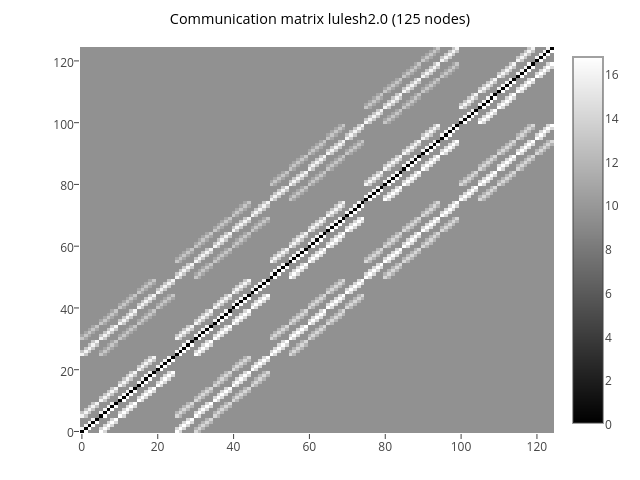
\includegraphics[scale=0.4]{cm_lulesh2_125}
\caption{Communication matrix with 125 ranks in the network.}
\label{fig:1}
\end{figure}

\section{experiment and results}

We chose a scientific application called \textit{kernel conjugate gradient} to show how to generate clusters of ranks using community detection algorithms starting from a communication matrix. This application is describes next.

\subsection{Kernel Conjugate Gradient}

The application \textit{kernel conjugate gradient} belongs to the NAS parallel benchmarks. This application solve an unstructured sparse linear system by the conjugate gradient method. A conjugate gradient method is used to compute an approximation to the smallest eigenvalue of a large sparse symmetric positive definite matrix. This kernel is typical of unstructured grid computations because it tests irregular long distance communication, employing unstructured matrix vector multiplication. This benchmark uses the inverse power method to find an estimate of the largest eigenvalue of a symmetric positive definite sparse matrix with a random pattern of nonzeros \cite{cg}.

\subsection{Detecting Communities in kernel conjugate gradient}

We applied the \textit{fast greedy} algorithm to the communication matrix of the kernel conjugate gradient to see what groups are generated by the \textit{fast greedy} algorithm. The experiments were executed changing the number of processors to know what was the effect of that. The results are shown in Figure \ref{fig:2}. Each element in the axis represents a rank of the application and each color in the figure represents a community detected within the network by the algorithm. 

It can be seen in Figure \ref{fig:2} that the elements of each community are consecutive ranks. Also, it is notable that these communities are very symmetric because each of them has pretty much the same number of elements. The only exception to this rule is the detection of communities for 512 ranks. In this case, there are some communities with different size. This is shown in Figure \ref{fig:3}, where x-axis represent the number of the community and y-axis represent the number of elements in the community. 

Based on Figures \ref{fig:2} and \ref{fig:3} is clear that the communities are well define and is clear how could be the split of the network.

\begin{table}[h!]
\begin{center}
 \begin{tabular}{||c || c|| c ||} 
 \hline
 Number of processors&Modularity&Number of communities \\ [0.5ex] 
 \hline\hline
64 &	0.65 & 8	\\
 \hline
128	&	0.69 & 8\\
 \hline
256	&	0.75 & 16\\
 \hline
512	& 0.77 & 16\\
 \hline
\end{tabular}
 \caption{Modularity and number of communities to each number of processors in kernel conjugate gradient.}
 \label{table:1}
\end{center}
\end{table}

Table \ref{table:1} shows the modularity and number of communities detected by the \textit{fast greedy} algorithm for different number of processes. The results shown that when we added more processes in the application, the number of groups and the modularity grew up. Because the community detection algorithms use modularity, this measure can be use to compare the results. Some authors have mentioned that a good value of modularity is usually between 0.3 and 0.7 \cite{NewGir04,Clauset}. As the results are in that range these groups are good to describe a partition of the network that maximize intracluster communication and minimize intercluster communication.

\begin{figure*}[h!]
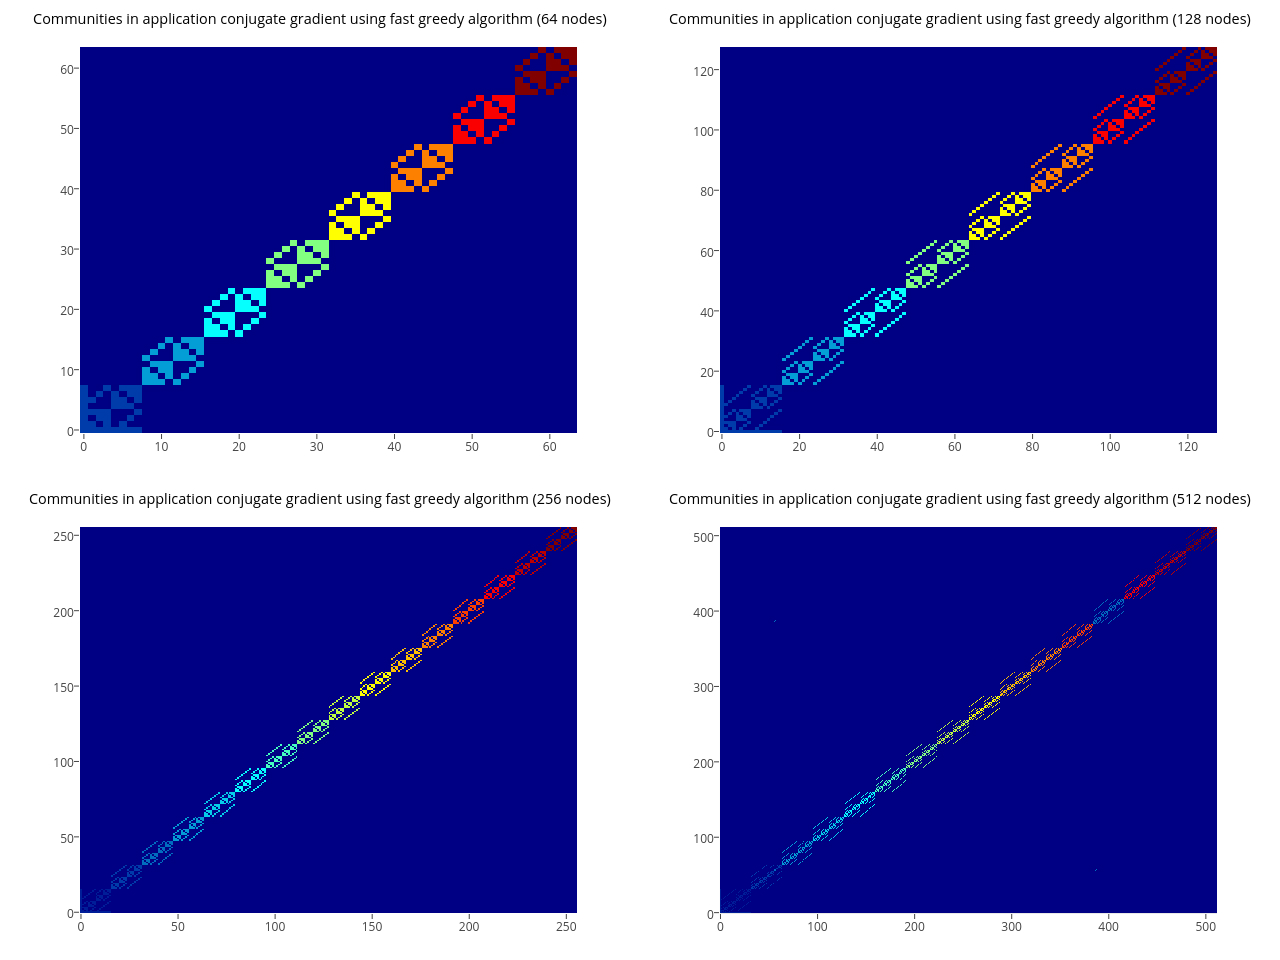
\includegraphics[width=\textwidth, height=10cm]{com_algorithms_cg_fg_64_128_256_512}
\caption{Communities detected by the fast greedy algorithm on different number of processors in conjugate gradient.}
\label{fig:2}
\end{figure*}


\begin{figure*}[h!]
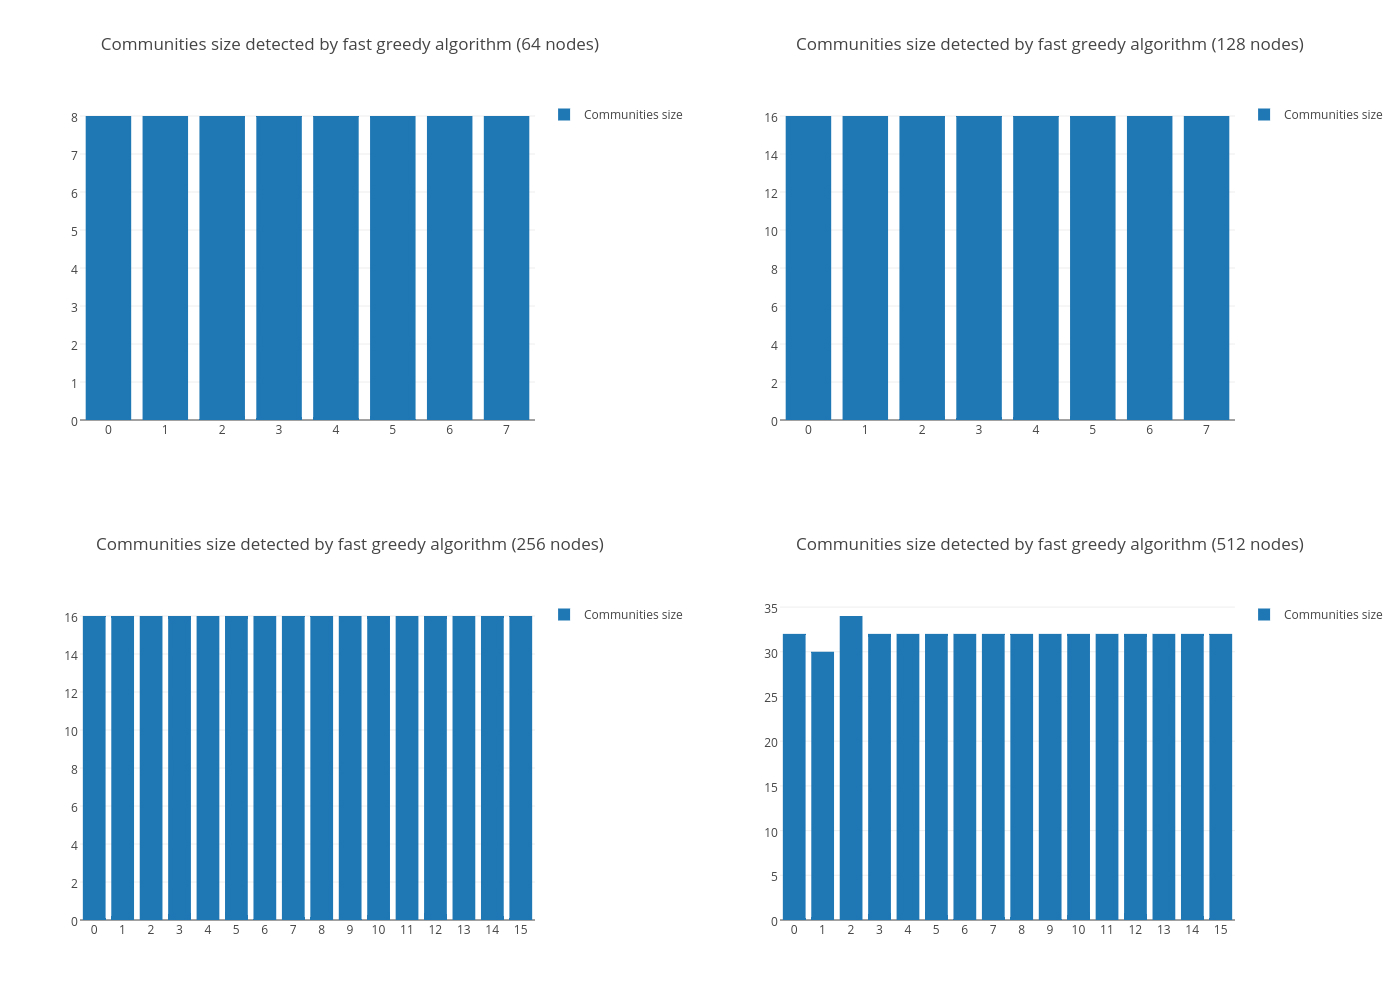
\includegraphics[width=\textwidth, height=10cm]{number_communities_cg_fg_64_128_256_512}
\caption{Communities's size in conjugate gradient using fast greedy algorithm.}
\label{fig:3}
\end{figure*}


\section{Conclusion}

We applied the \textit{fast greedy} community detection algorithm to the communication matrix of \textit{kernel conjugate gradient}. The analysis showed well define communities that can help to split the network in groups of ranks that could be together to improve latency of the communication. Also, some of the partitions of this network had a good modularity between 0.6 and 0.7.

The results showed that the \textit{fast greedy} algorithm detected communities with good modularity and structure. Further, this algorithm is stable because it detected good communities when the number of processes in the network was changed. 

The application showed well defined communities and it was easy to find this communities with detection algorithms. Besides, in some cases the communities detected were symmetric because they had the same number of elements.

The communication matrix was proven to give insight into communication in parallel applications.

\section{Future Work}

One important thing to do is to use the kernel conjugate gradient and apply the \textit{fast greedy} algorithm in a network with more nodes to see if the behavior is maintained. On the other hand, it is important to explore more applications and apply these methods in real applications that are been using in real time to know if the work proposed can be applied in the real life. 

After applying these algorithms to a real applications, it might be interesting to implement a special network that could represent exactly the communities detected by the algorithms and see if the split of the network can help to improve the application performance.

In the future, it would be interesting to add more point-to-point and collective operations to identify how this can affect the detection of communities. Further, in some cases it would be interesting to filter the operations used to detect the communities to identify if some could be feeding noise to the algorithms.

Finally, it is important to try with more community detection algorithms to compare their results and see if it is possible to get better or different communities and have different point of views of how the network can be divided in groups of processes to achieve better performance in communication.

\bibliographystyle{IEEEtran}
\bibliography{references.bib}


\end{NoHyper}
% that's all folks
\end{document}


